\section{Binary Encodings} 
  
  We have motivated the need for \textit{binary} encodings through the construction of the transistor. In retrospect, we can therefore see why we want to develop a theory around \hyperref[th-binary_motivation]{binary alphabets} in $\{0, 1\}^\ast$. Now that we know how to work with them, the remaining task of encoding elements of an arbitrary set $S \to \{0, 1\}^\ast = \sqcup_n \{0, 1\}^n$ is mathematically trivial. 

  \begin{definition}[Representation Scheme]
    A \textbf{representation scheme} is an encoding of an object $s$ to a unique binary string $E(s) \in \{0,1\}^\ast$. It is an injective function 
    \begin{equation}
      E: X \longrightarrow \{0,1\}^\ast
    \end{equation}
  \end{definition}

  Therefore, when we say that a program $P$ takes $x$ as an input, we really mean that $P$ takes as input the \textit{representation of $x$} as a binary string.  

  Since $\{0, 1\}^\ast$ is \hyperref[set-def:countable]{countable}, there always exists an injective map $f: S \to \{0, 1\}^\ast$ as long as $S$ is at most countable. But in practicality, we would like to find a good encoding that is easy to work with. Throughout this chapter, we will consider different sets $S$ and introduce the standard encodings for each set. 

  In order to get into memory, it is helpful to know the theory behind how primitive types are stored in memory.  

  \begin{definition}[Collections of Bits]
    There are many words that are used to talk about values of different data types: 
    \begin{enumerate}
      \item A \textbf{bit} (b) is either $0$ or $1$. 
      \item A \textbf{Hex} (x) is a collection of 4 bits, with a total of $2^4 = 16$ possible values, and this is used since it is easy to read for humans. 
      \item A \textbf{Byte} (B) is a collection of 8 bits or 2 hex, with a total of $2^8 = 256$ possible values, and most computers will work with Bytes as the smallest unit of memory. 
    \end{enumerate}
  \end{definition}

\subsection{Naturals/Unsigned and Integers/Signed}

  \begin{definition}[Representation of the Naturals]
    A representation for natural numbers (note that in this context, $0 \in \mathbb{N}$) is the (non-surjective) regular binary representation denoted
    \begin{equation}
      NtS: \mathbb{N} \longrightarrow \{0,1\}^\ast \;\;\;\; (NtS= \text{ "Naturals to Strings"})
    \end{equation}
    recursively defined as 
    \[NtS(n) = \begin{cases}
    0 & n = 0 \\
    1 & n = 1 \\
    NtS(\left \lceil{n/2}\right \rceil parity(n) & n > 1 
    \end{cases}\]
    where given strings $x, y \in \{0,1\}^\ast$, $xy$ denotes the concatenation of $x$ and $y$, and $parity: \mathbb{N} \longrightarrow \{0,1\}^\ast$ is defined 
    \[parity(n) = \begin{cases}
    0 & n $\text{ is even}$ \\
    1 & n $\text{ is odd}$
    \end{cases}\]
    Since $NtS$ in injective, its inverse $StN: \mathrm{Im}{NtS} \subset \{0,1\}^\ast \longrightarrow \mathbb{N}$ is well-defined. 
  \end{definition}

  \begin{definition}[Representation of the Integers]
    To construct a representation scheme for $\mathbb{Z}$, we can just add one more binary digit to represent the sign of the number. The binary representation $ZtS: \mathbb{Z} \longrightarrow \{0, 1\}^\ast$ is defined
    \[ZtS(m) = \begin{cases}
    0\, NtS(m) & m \geq 0 \\
    1 \, NtS(-m) & m < 0
    \end{cases}\]
    where $NtS$ is defined as before. Again this function must be injective but need not be surjective. 
  \end{definition}

  The most primitive things that we can store are integers. Let us talk about how we represent some of the simplest primitive types in C: unsigned short, unsigned int, unsigned long, unsigned long long.

  \begin{definition}[Unsigned Integer Types in C]
    In C, there are several integer types. We use this hierarchical method to give flexibility to the programmer on the size of the integer and whether it is signed or not. 
    \begin{enumerate} 
      \item An \textbf{unsigned short} is 2 bytes long and can be represented as a 4-digit hex or 16 bits, with values in $[0:65,535]$. Therefore, say that we have 
      \item An \textbf{unsigned int} is 4 bytes long and can be represented as an 8-digit hex or 32 bits, with values in $[0:4,294,967,295]$. 
      \item An \textbf{unsigned long} is 8 bytes and can be represented as an 16-digit hex or 64 bits, but they are only guaranteed to be stored in 32 bits in other systems. 
      \item An \textbf{unsigned long long} is 8 bytes and can be represented as an 16-digit hex or 64 bits, and they are guaranteed to be stored in 64 bits in other systems. 
    \end{enumerate} 
  \end{definition}

  \begin{theorem}[Bit Representation of Unsigned Integers in C]
    To encode a signed integer in bits, we simply take the binary expansion of it. 
    \begin{figure}[H]
      \centering 
      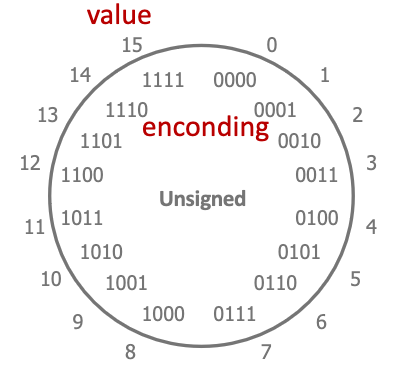
\includegraphics[scale=0.4]{img/unsigned_encoding.png}
      \caption{Unsigned encoding of 4-bit integers in C. } 
      \label{fig:unsigned_encoding}
    \end{figure}
  \end{theorem}

  \begin{example}[Bit Representation of Unsigned Integers in C]
    We can see for ourselves how these numbers are represented in bits. Printing the values out in binary requires to make new functions, but we can easily convert from hex to binary. 

    \noindent\begin{minipage}{.5\textwidth}
    \begin{lstlisting}[]{Code}
      int main() { 

        unsigned short x = 13; 
        unsigned int y = 256;

        printf("%x\n", x);
        printf("%x\n", y);

        return 0; 
      }
    \end{lstlisting}
    \end{minipage}
    \hfill
    \begin{minipage}{.49\textwidth}
    \begin{lstlisting}[]{Output}
      d
      100 
      .
      .
      .
      .
      .
      .
      .
      .
    \end{lstlisting}
    \end{minipage}
  \end{example}

  So far, the process of converting unsigned numbers to bits seemed simple. Now let's introduce signed integers. 

  \begin{definition}[Signed Integer Types in C]
    In C, there are several signed integer types. We use this hierarchical method to give flexibility to the programmer on the size of the integer and whether it is signed or not. 
    \begin{enumerate} 
      \item A \textbf{signed short} is 2 bytes long and can be represented as a 4-digit hex or 16 bits, with values in $[-32,768: 32,767]$. 
      \item A \textbf{signed int} is 4 bytes long and can be represented as an 8-digit hex or 32 bits, with values in $[-2,147,483,648: 2,147,483,647]$. 
      \item A \textbf{signed long} is 8 bytes and can be represented as an 16-digit hex or 64 bits, but they are only guaranteed to be stored in 32 bits in other systems. 
      \item A \textbf{signed long long} is 8 bytes and can be represented as an 16-digit hex or 64 bits, and they are guaranteed to be stored in 64 bits in other systems. 
    \end{enumerate}
  \end{definition}

  To store signed integers, it is intuitive to simply take the first (left-most) bit and have that be the sign. Therefore, we lose one significant figure but gain information about the sign. However, this has some problems: first, there are two representations of zeros: $-0$ and $+0$. Second, the continuity from $-1$ to $0$ is not natural. It is best explained through an example, which doesn't lose much insight into the general case. 

  \begin{example}[Problems with the Signed Magnitude]
    Say that you want to develop the signed magnitude representation for 4-bit integers in C. Then, you can imagine the following diagram to represent the numbers. 
    \begin{figure}[H]
      \centering 
      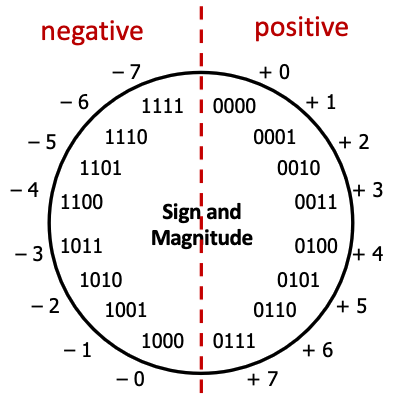
\includegraphics[scale=0.4]{img/signed_magnitude_encoding.png}
      \caption{Signed magnitude encoding of 4-bit integers in C.} 
      \label{fig:signed_magnitude_encoding}
    \end{figure}
    You can see that there are some problems: 
    \begin{enumerate}
      \item There are two representations for $0$, which is 0000 and 1000. 
      \item -1 (1001) plus 1 becomes -2 (1010). 
      \item The lowest number -7 (1111) plus 1 goes to 0 (0000) when it should go to -6 (1100). 
      \item The highest number 7 (0111) plus 1 goes to 0 (1000). 
    \end{enumerate}
  \end{example}

  An alternative way is to use the two's complement representation, which solves both problems and makes it more natural. 

  \begin{theorem}[Bit Representation of Signed Integers in C]
    The \textbf{two's complement} representation is a way to represent signed integers in binary. It is defined as follows. Given that you want to store a decimal number $p$ in $n$ bits, 

    \begin{enumerate}
      \item If $p$ is positive, then take the binary expansion of that number, which should be at most $n-1$ bits (no overflow), pad it with $0$s on the left. 
      \item If $p$ is negative, then you can do two things: First, take the binary expansion of the positive number, flip all the bits, and add 1. Or second, represent $p = q - 2^n$, take the binary representation of $q$ in $n-1$ bits, and add a $1$ to the left. 
    \end{enumerate}
    If you have a binary number $b = b_{n}b_{n-1}\cdots b_1$ then to convert it to a decimal number, you simply calculate 
    \begin{equation}
      q = -b_{n}2^{n-1} + b_{n-1}2^{n-2} + \cdots + b_1
    \end{equation}
    \begin{figure}[H]
      \centering 
      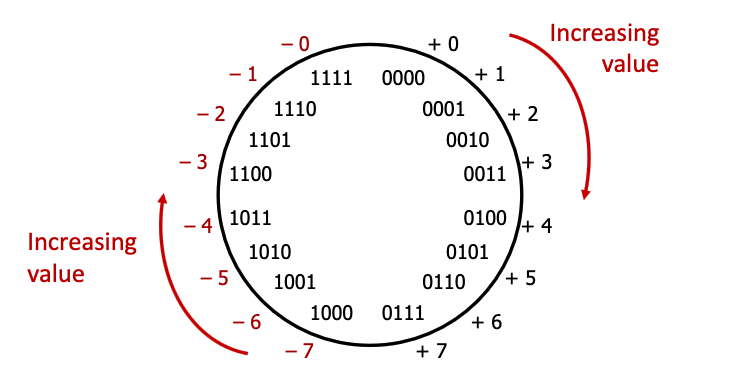
\includegraphics[scale=0.4]{img/twos_complement_encoding.png}
      \caption{Two's complement encoding of 4-bit integers in C.} 
      \label{fig:twos_complement_encoding}
    \end{figure}
  \end{theorem}

  \begin{example}[Bit Representation of Signed Integers in C]
    We can see for ourselves how these numbers are represented in bits. 

    \noindent\begin{minipage}{.5\textwidth}
    \begin{lstlisting}[]{Code}
      int main() { 

        short short_pos = 13; 
        short short_neg = -25; 
        int int_pos = 256;
        int int_neg = -512; 

        printf("%x\n", short_pos);
        printf("%x\n", short_neg);
        printf("%x\n", int_pos);
        printf("%x\n", int_neg);

        return 0; 
      }
    \end{lstlisting}
    \end{minipage}
    \hfill
    \begin{minipage}{.49\textwidth}
    \begin{lstlisting}[]{Output}
      d
      ffe7
      100
      ffffffe00
      .
      .
      .
      .
      .
      .
      .
      .
      .
      .
    \end{lstlisting}
    \end{minipage}
  \end{example}

  \begin{figure}[H]
    \centering 
    \noindent\begin{minipage}{.5\textwidth}
    \begin{lstlisting}[]{Code}
      #include<stdio.h>
      #include<stdbool.h>

      int main() {
        printf("%lu\n", sizeof(bool)); 
        printf("%lu\n", sizeof(short)); 
        printf("%lu\n", sizeof(int)); 
        printf("%lu\n", sizeof(long)); 
        printf("%lu\n", sizeof(long long)); 
        return 0; 
      }
    \end{lstlisting}
    \end{minipage}
    \hfill
    \begin{minipage}{.49\textwidth}
    \begin{lstlisting}[]{Output}
      1
      2
      4
      8
      8
      .
      .
      .
      .
      .
      .
    \end{lstlisting}
    \end{minipage}
    \caption{Size of various integer types in C with the \texttt{sizeof}.} 
    \label{fig:integer_size}
  \end{figure}


  \subsubsection{Arithmetic Operations on Binary Numbers}

    \begin{theorem}[Inversion of Binary Numbers]
      Given a binary number $p$, to compute $-p$, simply invert the bits and add 1.
    \end{theorem}

    \begin{theorem}[Addition and Subtraction of Binary Numbers]
      Given two binary numbers $p$ and $q$. 
      \begin{enumerate}
        \item To compute $p + q$, simply add the numbers together as you would in base 10, but carry over when the sum is greater than 1. 
        \item To compute $p - q$, you can invert $q$ to $-q$ and compute $p + (-q)$. 
      \end{enumerate}
    \end{theorem}

    % TODO: Bitshift and Bitwise Operations

\subsection{Rationals and Countable Sets}
  
  When representing rational numbers, we cannot simply concatenate the numerator and denominator as such
  \[a/b \mapsto ZtS(a) \, ZtS(b)\]
  since this map is not surjective (and may overlap with other integers). 

  \begin{definition}[Representation of Rationals]
    To represent a rational number $a/b$, we create a separator symbol $|$ and map the rational number as below in the alphabet $\{0, 1, |\}$. 
    \[q: a/b \mapsto ZtS(a) | ZtS(b)\]
    Then, we use a second map that goes through each digit in $z$ and is defined 
    \[p: \{0, 1, |\} \longrightarrow \{00,11,01\} \subset \{0, 1\}^2, \; p(n) = \begin{cases}
    00 & n = 0 \\
    11 & n = 1 \\
    01 & n = |
    \end{cases}\]
    Therefore, $p$ maps the length $n$ string $z \in \{0, 1\}^\ast$ to the length $2n$ string $\omega \in \{0, 1\}^\ast$. The representation scheme for $\mathbb{Q}$ is simply 
    \[QtS \equiv p \circ q\]
  \end{definition}

  \begin{example}
  Given the rational number $-5/8$,
  \[\frac{-5}{8} \mapsto 1101|01000 \mapsto 11110011010011000000\]
  \end{example}

  This same idea of using separators and compositions of injective functions can be used to represent arbitrary $n$-tuples of strings (since a finite Cartesian product of countable sets is also countable). 

  \begin{theorem}[Representation of Vectors]
    All vectors, matrices, and tensors over the field $\mathbb{Q}$ are representable. 
  \end{theorem}
  \begin{proof}
    For vectors, we can simply create another separator symbol $\cdot$ and have the initial mapping $q$ map to a string over the alphabet $\{0, 1, |, \cdot\}$, which injectively maps to $\{00, 01, 10, 11\}$. 
    For tensors, create more separator symbols and map them to a sufficiently large set (which can be extended arbitrarily). For example, to perhaps $\{000, 001, ..., 111\}$. 

  \end{proof}

  \begin{corollary}[Representation of Graphs]
    Directed graphs, which can be represented with their adjacency matrices, can therefore be represented with binary strings. 
  \end{corollary}

  \begin{theorem}[Representation of Images]
    Every finite-resolution image can be represented as a binary number. 
  \end{theorem}
  \begin{proof}
    Since we can interpret each image as a matrix where each element (a pixel) is a color, and since each color can be represented as a 3-tuple of rational numbers corresponding to the intensities of red, green, and blue (for humans, we can restrict it to three primary colors), all images can eventually be decomposed into binary strings. 
  \end{proof}

\subsection{Floats} 

  \begin{theorem}[Representation of Reals]
    There exists no representation of the reals
    \begin{equation}
      NtR: \mathbb{R} \longrightarrow \{0, 1\}^\ast
    \end{equation}
  \end{theorem}
  \begin{proof}
    By Cantor's theorem, the reals are uncountable. That is, there does not exist a surjective function $NtR: \mathbb{N} \longrightarrow \mathbb{R}$. The implies the nonexistence of an injective inverse; that is, there does not exist an injective function 
    \[RtS: \mathbb{R} \longrightarrow \{0,1\}^\ast\]
  \end{proof}

  However, since $\mathbb{Q}$ is dense in $\mathbb{R}$, we can approximate every real number $x$ by a rational number $a/b$ to arbitrary accuracy. There are multiple ways to construct these approximations (decimal approximation up to $k$th digit, finite continued fractions, truncated infinite series, etc.), but computers use the \textit{floating-point approximation}. 

  \begin{definition}[Floating-Point Representation]
    The \textbf{floating-point representation scheme} of a real number $x \in \mathbb{R}$ is its approximation as a number of the form 
    \[\sigma b \cdot 2^e\]
    where $\sigma \in \{0, 1\}$ determines the sign of the representation of $x$, $e$ is a (potentially negative) integer, and $b$ is a rational number between $1$ and $2$ expressed as a binary fraction 
    \[1.b_0 b_1 b_2 ... b_k = 1 + \frac{b_1}{2} + \frac{b_2}{4} + ... + \frac{b_k}{2^k}, \;\; b_i \in \{0,1\}\]
    where the number $k$ is fixed (determined by the desired accuracy; greater $k$ implies more digits and better accuracy). The $\sigma b \cdot 2^e$ closest to $x$ is the \textit{floating-point representation}, or \textit{approximation}, of $x$. We can think of $\sigma$ determining the sign, $e$ the order of magnitude (in base 2) of $x$, and $b$ the value of the number scaled down to a value in $[1,2)$, called the \textit{mantissa}. 
  \end{definition}

  \begin{definition}[Floating Point Types in C]
    In C, there are several floating point types. We use this hierarchical method to give flexibility to the programmer on the size of the integer and whether it is signed or not. 
    \begin{enumerate} 
      \item A \textbf{float} is 4 bytes long and can be represented as an 8-digit hex or 32 bits, with values in $[1.2 \times 10^{-38}: 3.4 \times 10^{38}]$. 
      \item A \textbf{double} is 8 bytes long and can be represented as an 16-digit hex or 64 bits, with values in $[2.3 \times 10^{-308}: 1.7 \times 10^{308}]$. 
      \item A \textbf{long double} is 8 bytes and can be represented as an 16-digit hex or 64 bits, but they are only guaranteed to be stored in 80 bits in other systems. 
    \end{enumerate}
  \end{definition}

  \begin{theorem}[Bit Representation of Floating Point Types in C]
    Floats are actually like signed magnitude. We have 
    \begin{equation} 
      (-1)^n \times 2^{e - 127} \times 1.s
    \end{equation}

    \begin{figure}[H]
      \centering 
      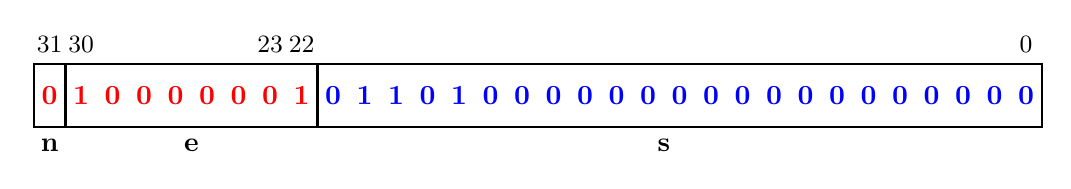
\begin{tikzpicture}[scale=0.8]
        % Draw the main box
        \draw[thick] (0,0) rectangle (16,1);
        
        % Vertical dividers
        \draw[thick] (0.5,0) -- (0.5,1);
        \draw[thick] (4.5,0) -- (4.5,1);
        
        % Bit numbers at top
        \node at (0.25,1.3) {\small 31};
        \node at (0.75,1.3) {\small 30};
        \node at (3.75,1.3) {\small 23};
        \node at (4.25,1.3) {\small 22};
        \node at (15.75,1.3) {\small 0};
        
        % Sign bit (red)
        \node[red] at (0.25,0.5) {\textbf{0}};
        
        % Exponent bits (red)
        \node[red] at (0.75,0.5) {\textbf{1}};
        \node[red] at (1.25,0.5) {\textbf{0}};
        \node[red] at (1.75,0.5) {\textbf{0}};
        \node[red] at (2.25,0.5) {\textbf{0}};
        \node[red] at (2.75,0.5) {\textbf{0}};
        \node[red] at (3.25,0.5) {\textbf{0}};
        \node[red] at (3.75,0.5) {\textbf{0}};
        \node[red] at (4.25,0.5) {\textbf{1}};
        
        % Mantissa bits (blue)
        \node[blue] at (4.75,0.5) {\textbf{0}};
        \node[blue] at (5.25,0.5) {\textbf{1}};
        \node[blue] at (5.75,0.5) {\textbf{1}};
        \node[blue] at (6.25,0.5) {\textbf{0}};
        \node[blue] at (6.75,0.5) {\textbf{1}};
        \node[blue] at (7.25,0.5) {\textbf{0}};
        \node[blue] at (7.75,0.5) {\textbf{0}};
        
        % Remaining zeros in light blue
        \foreach \x in {8.25,8.75,9.25,9.75,10.25,10.75,11.25,11.75,12.25,12.75,13.25,13.75,14.25,14.75,15.25,15.75} {
          \node[blue] at (\x,0.5) {\textbf{0}};
        }
        
        % Labels below
        \node at (0.25,-0.3) {\textbf{n}};
        \node at (2.5,-0.3) {\textbf{e}};
        \node at (10,-0.3) {\textbf{s}};
      \end{tikzpicture}
      \caption{32-bit representation of floats.} 
    \end{figure}

    Doubles encode 64 bits, so now we have exponent having 11 bits (so bias is not 1023) and 52 bits for mantissa. 
  \end{theorem}

\subsection{Characters}

  \begin{definition}[Booleans in C]
    The most basic type is the boolean, which is simply a bit. In C, it is represented as \texttt{bool}, and it is either \texttt{true} (1) or \texttt{false} (0). 
  \end{definition}

  We can manually check the size of the boolean type in C with the following code. 

  \begin{figure}[H]
    \centering 
    \noindent\begin{minipage}{.5\textwidth}
    \begin{lstlisting}[firstnumber=1]{Code}
      #include<stdio.h>
      #include<stdbool.h>

      int main() {
        printf("%lu\n", sizeof(bool)); 
        return 0; 
      }
    \end{lstlisting}
    \end{minipage}
    \hfill
    \begin{minipage}{.49\textwidth}
    \begin{lstlisting}[]{Output}
      1
      .
      .
      .
      .
      .
      .
    \end{lstlisting}
    \end{minipage}
    \caption{We can verify the size of various primitive data types in C with the \texttt{sizeof} operator.} 
    \label{fig:boolean_size}
  \end{figure}

  Note that \textbf{it does not make sense to have a string without knowing what encoding it uses}. We can't just assume that every plaintext is in ASCII, since there are hundreds of extended ASCII encodings. If you have a string, in memory, in a file, or in an email message, you have to know what encoding it is in or you cannot interpret it or display it to users correctly. 

  For example, when you are sending an email, Gmail is the only client that automatically converts your text to UTF-8, regardless of what you set in the header. The browser also uses a certain encoding, which can be accessed (and changed) under the "view" tab. 

  \subsubsection{ASCII}

    \begin{definition}[ASCII]
      The \textbf{ASCII} (also called US-ASCII) code, which stands for American Standard Code for Information Interchange is a $7$ bit character code where every single bit represents a unique character. ASCII codes represent text in computers, telecommunications equipment, and other devices. Most modern character-encoding schemes are based on ASCII, although they support many additional characters.

      The first 32 characters are called the \textit{control characters}: codes originally intended not to represent printable information, but rather to control devices (such as printers) that make use of ASCII, or to provide meta-information about data streams. For example, character 10 (decimal) represents the "line feed" function (which causes a printer to advance its paper) and character 8 represents "backspace." Except for the control characters that prescribe elementary line-oriented formatting, ASCII does not define any mechanism for describing the structure or appearance of text within a document. 
      \begin{center}
      \scalebox{0.8}{%
      \begin{tabular}{ |c|c|c|c|c|l| } 
        \hline
        Dec & Oct & Hex & Bin & Symbol & Description\\ 
        \hline
        0 & 000& 00& 0000000 & NULL & Null char\\ 
        1 & 001&01&0000001 & SOH & Start of Heading \\
        2 & 002 & 02 & 0000010& STX & Start of Text \\
        3 & 003 & 03 & 0000011&ETX & End of Text \\
        4 & 004 & 04 & 0000100 & EOT & End of Transmission \\
        5 & 005 & 05 & 0000101 & ENQ & Enquiry \\
        6 & 006 & 06 & 0000110 & ACK & Acknowledgement \\
        7 & 007 & 07 & 0000111 & BEL & Bell \\
        8 & 010 & 08 & 0001000 & BS & Back Space\\
        9 & 011 & 09 & 0001001 & HT & Horizontal Tab \\
        10 & 012 & 0A & 0001010 & LF & Line Feed \\
        11 & 013 & 0B & 0001011 & VT & Vertical Tab \\
        12 & 014 & 0C & 0001100 & FF & Form Feed\\
        13 & 015 & 0D & 0001101 & CR & Carriage Return \\
        14 & 016 & 0E & 0001110 & SO & Shift Out/X-On\\
        15 & 017 & 0F & 0001111 & SI & Shift In/X-Off\\
        16 & 020 & 10 & 0010000 & DLE & Data Line Escape\\
        17 & 021 & 11 & 0010001 & DC1 & Device Control 1\\
        18 & 022 & 12 & 0010010 & DC2 & Device Control 2\\
        19 & 023 & 13 & 0010011 & DC3 & Device Control 3\\
        20 & 024 & 14 & 0010100 & DC4 & Device Control 4 \\
        21 & 025 & 15 & 0010101 & NAK & Negative Acknowledgement\\
        22 & 026 & 16 & 0010110 & SYN & Synchronous Idle \\
        23 & 027 & 17 & 0010111 & ETB & End of Transmit Block\\
        24 & 030 & 18 & 0011000 & CAN & Cancel\\
        25 & 031 & 19 & 0011001 & EM & End of Medium\\
        26 & 032 & 1A & 0011010 & SUB & Substitute\\
        27 & 033 & 1B & 0011011 & ESC & Escape\\
        28 & 034 & 1C & 0011100 & FS & File Separator \\
        29 & 035 & 1D & 0011101 & GS & Group Separator\\
        30 & 036 & 1E & 0011110 & RS & Record Separator \\
        31 & 037 & 1F & 0011111 & US & Unit Separator\\
        \hline
      \end{tabular}}
      \end{center}

      The rest of the characters are the ASCII printable characters. 

      \scalebox{0.8}{%
      \begin{tabular}{ |c|c|c|c|c|l|c|c|c|c|c|l| } 
        \hline
        Dec & Oct & Hex & Bin & Sym & Description & Dec & Oct & Hex & Bin & Sym & Description \\
        \hline
        32 & 040 & 20& 0100000 &   & Space & 80 & 120 & 50& 1010000 &P&Uppercase P\\
        33 & 041 & 21& 0100001 & ! & Exclamation & 81 & 121 & 51& 1010001 &Q&Uppercase Q\\
        34 & 042 & 22& 0100010 & " & Double quotes & 82 & 122 & 52& 1010010 &R&Uppercase R\\
        35 & 043 & 23& 0100011 & \# & Number & 83 & 123 & 53& 1010011 &S&Uppercase S\\
        36 & 044 & 24& 0100100 & \$ & Dollar & 84 & 124 & 54& 1010100 &T&Uppercase T\\
        37 & 045 & 25& 0100101 & \% & Per cent sign & 85 & 125 & 55& 1010101 &U&Uppercase U\\
        38 & 046 & 26& 0100110 & \& & Ampersand & 86 & 126 & 56& 1010110 &V&Uppercase V\\
        39 & 047 & 27& 0100111 & ' &Single quote & 87 & 127 & 57& 1010111 &W&Uppercase W\\
        40 & 050 & 28& 0101000 & ( & Open paren.& 88 & 130 & 58& 1011000 &X&Uppercase X\\
        41 & 051 & 29& 0101001 & ) & Closed paren.& 89 & 131 & 59& 1011001 &Y&Uppercase Y\\
        42 & 052 & 2A& 0101010 & * & Asterisk & 90 & 132 & 5A& 1011010 &Z&Uppercase Z\\
        43 & 053 & 2B& 0101011 & + & Plus & 91 & 133 & 5B& 1011011 & [ & Opening bracket\\
        44 & 054 & 2C& 0101100 & , & Comma & 92 & 134 & 5C& 1011100 & \textbackslash & Backslash\\
        45 & 055 & 2D& 0101101 & - & Hyphen & 93 & 135 & 5D& 1011101 & ] & Closing bracket\\
        46 & 056 & 2E& 0101110 & . &Period & 94 & 136 & 5E& 1011110 & \string^ & Caret\\
        47 & 057 & 2F& 0101111 & / & Slash & 95 & 137 & 5F& 1011111 & \_ & Underscore\\
        48 & 060 & 30& 0110000 & 0 & Zero & 96 & 140 & 60& 1100000 &`&Grave accent\\
        49 & 061 & 31& 0110001 & 1 & One & 97 & 141 & 61& 1100001 &a& Lowercase a\\
        50 & 062 & 32& 0110010 & 2 & Two & 98 & 142 & 62& 1100010 &b&Lowercase b\\
        51 & 063 & 33& 0110011 & 3 & Three & 99 & 143 & 63& 1100011 &c&Lowercase c\\
        52 & 064 & 34& 0110100 & 4 & Four & 100 & 144 & 64& 1100100 &d&Lowercase d\\
        53 & 065 & 35& 0110101 & 5 & Five & 101 & 145 & 65& 1100101 &e&Lowercase e\\
        54 & 066 & 36& 0110110 & 6 & Six & 102 & 146 & 66& 1100110 &f&Lowercase f\\
        55 & 067 & 37& 0110111 & 7 & Seven & 103 & 147 & 67 &1100111 &g&Lowercase g\\
        56 & 070 & 38& 0111000 & 8 & Eight & 104 & 150 & 68& 1101000 &h&Lowercase h\\
        57 & 071 & 39& 0111001 & 9 & Nine & 105 & 151 & 69& 1101001 &i&Lowercase i\\
        58 & 072 & 3A& 0111010 & : & Colon & 106 & 152 & 6A& 1101010 &j&Lowercase j\\
        59 & 073 & 3B& 0111011 & ; & Semicolon & 107 & 153 & 6B& 1101011 &k&Lowercase k\\
        60 & 074 & 3C& 0111100 & < & Less than & 108 & 154 & 6C& 1101100 &l&Lowercase l\\
        61 & 075 & 3D& 0111101 & = & Equals & 109 & 155 & 6D& 1101101 &m&Lowercase m\\
        62 & 076 & 3E& 0111110 & > & Greater than & 110 & 156 & 6E& 1101110 &n&Lowercase n\\
        63 & 077 & 3F& 0111111 & ? & Question mark & 111 & 157 & 6F& 1101111 &o&Lowercase o\\
        64 & 100 & 40& 1000000 & @ & At symbol & 112 & 160 & 70& 1110000 &p&Lowercase p\\
        65 & 101 & 41& 1000001 & A & Uppercase A & 113 & 161 & 71& 1110001 &q&Lowercase q\\
        66 & 102 & 42& 1000010 & B& Uppercase B & 114 & 162 & 72& 1110010 &r&Lowercase r\\
        67 & 103 & 43& 1000011 &C&Uppercase C & 115 & 163 & 73& 1110011 &s&Lowercase s\\
        68 & 104 & 44& 1000100 &D&Uppercase D & 116 & 164 & 74& 1110100 &t&Lowercase t\\
        69 & 105 & 45& 1000101 &E&Uppercase E & 117 & 165 & 75& 1110101 &u&Lowercase u\\
        70 & 106 & 46& 1000110 &F&Uppercase F & 118 & 166 & 76& 1110110 &v&Lowercase v\\
        71 & 107 & 47& 1000111 &G&Uppercase G & 119 & 167 & 77& 1110111 &w&Lowercase w\\
        72 & 110 & 48& 1001000 &H&Uppercase H & 120 & 170 & 78& 1111000 &x&Lowercase x\\
        73 & 111 & 49& 1001001 &I&Uppercase I & 121 & 171 & 79& 1111001 &y&Lowercase y\\
        74 & 112 & 4A& 1001010 &J&Uppercase J & 122 & 172 & 7A& 1111010 &z&Lowercase z\\
        75 & 113 & 4B& 1001011 &J&Uppercase K & 123 & 173 & 7B& 1111011 &\{& Opening brace\\
        76 & 114 & 4C& 1001100 &L&Uppercase L & 124 & 174 & 7C& 1111100 &|& Vertical bar\\
        77 & 115 & 4D& 1001101 &M&Uppercase M & 125 & 175 & 7D& 1111101 &\}& Closing brace\\
        78 & 116 & 4E& 1001110 &N&Uppercase N & 126 & 176 & 7E& 1111110 & $\sim$ & Tilde\\
        79 & 117 & 4F& 1001111 &O&Uppercase O & 127 & 177 & 7F& 1111111 & & Delete\\
        \hline
      \end{tabular}}
    \end{definition}

    The \textbf{Extended ASCII} (EASCII or high ASCII) character encodings are 8-bit or larger encodings that include the standard 7-bit ASCII characters, plus additional characters. Note that this does not mean that the standard ASCII coding has been updated to include more than 128 characters nor does it mean that there is an universal extension to the original ASCII coding. In fact, there are several (over 100) extended ASCII encodings. 

    With the creation of the 7-bit ASCII format, increased need for more letters and symbols (such as characters in other languages or more punctuation/mathematical symbols). With better computers and software, it became obvious that they could handle text that uses 256-character sets at almost no additional cost in programming or storage. The 8-bit format would allow ASCII to be used unchanged and provide 128 more characters. 

    But even 256 characters is still not enough to cover all purposes, all languages, or even all European languages, so the emergence of \textit{many} ASCII-derived 8-bit character sets was inevitable. Translating between these sets (\textit{transcoding}) is complex, especially if a character is not in both sets and was often not done, producing \textbf{mojibake} (semi-readable text resulting from text being decoded using an unintended character encoding. The result is a systematic replacement of symbols with completely unrelated ones, often from a different writing system). ASCII can also be used to create graphics, commonly called \textbf{ASCII art}. 

    But ASCII isn't enough. We have lots of languages with lots of characters that computers should ideally display. Unicode assigns each character a unique number, or code print. Computers deal with such numbers as bytes: 8-bit computers would treat an 8-bit byte as the largest numerical unit easily represented on the hardware, 16-bit computers would expand that to 2 bytes, and so forth. Old character encodings like ASCII are from the (pre-) 8-bit era, and try to cram the dominant language in computing at the time, i.e. English, into numbers ranging from 0 to 127 (7 bits). When ASCII got extended by an 8th bit for other non-English languages, the additional 128 numbers/code points made available by this expansion would be mapped to different characters depending on the language being displayed. The \textbf{ISO-8859} standards are the most common forms of this mapping: 
    \begin{enumerate}
      \item \textbf{ISO-8859-1}
      \item \textbf{ISO-8859-15}, also called \textbf{ISO-Latin-1}
    \end{enumerate}
    But that's not enough when you want to represent characters from more than one language, so cramming all available characters into a single byte just won't work. The following shows ways to do this (that is compatible with ASCII). 

  \subsubsection{ISO-10646, UCS}

    We can simply expand the value range by adding more bits. The UCS-2 uses 2 bytes (or 16 bits) and UCS-4 uses 4 bytes (32 bits). However, these codings suffer from inherently the same problem as ASCII and ISO-8859 standards, as their value range is still limited, even if the limit is vastly higher. Note that these encode from the ISO-10646, which defines several character encoding forms for the Universal Coded Character Set. 
    \begin{enumerate}
        \item UCS-2 can store $2^{16} = 65,536$ characters. 
        \item UCS-4 can store $2^{32} = 4,294,967,296$ characters. 
    \end{enumerate}
    Notice that UCS encoding has a fixed number of bytes per character, which means that UCS-2 stores each character in 2 bytes, and UCS-4 stores each character in 4 bytes. This is different from \textbf{UTF-8} encoding. 

    ISO 10646 and Unicode have an identical repertoire and numbers—the same characters with the same numbers exist on both standards, although Unicode releases new versions and adds new characters more often. Unicode has rules and specifications outside the scope of ISO 10646. ISO 10646 is a simple character map, an extension of previous standards like ISO 8859. In contrast, Unicode adds rules for collation, normalization of forms, and the bidirectional algorithm for right-to-left scripts such as Arabic and Hebrew. For interoperability between platforms, especially if bidirectional scripts are used, it is not enough to support ISO 10646; Unicode must be implemented.

  \subsubsection{Unicode, UTF-8}

    Unicode is the universal character encoding, maintained by Unicode Consortium, and it covers the characters for all the writing systems of the world, modern and ancient. It also includes technical symbols, punctuation, and many other characters used in writing text. As of Unicode Version 13.0, the Unicode standard contains 143,859 characters, stored in the format U+****, where **** is a number in hexadecimal notation. Notice that these ones are not fixed in the number of bits; that is, 
    \[\text{U+27BD and U+1F886}\]
    are perfectly viable representations of characters in Unicode. Even though only 143,859 characters are in use, Unicode currently allows for 1,114,112 ($16^5 + 16^4$) code values, and assigns codes covering nearly all modern text writing systems, as well as many historical ones and for many non-linguistic characters such as printer's dingbats, mathematical symbols, etc.

    \textit{Note that Unicode, along with ISO-10646, is a standard that assigns a name and a value (\textbf{Character Code} or \textbf{Code-Point}) to each character in its repertoire.} However, the Unicode format must be encoded in a binary format for the computer to understand. When you save a document, the text editor has to explicitly set its encoding to be UTF-8 (or whatever other format) the user wants it to be. Also, when a text editor program reads a file, it needs to select a text encoding scheme to decode it correctly. Even further, when you are typing and entering a letter, the text editor needs to know what scheme you use so that it will save it correctly. Therefore, \textit{UTF-8 encoding is a way to represent these characters digitally in computer memory.} The way that \textbf{UTF-8} encodes characters is with the following format:
    \begin{lstlisting}
    1st Byte    2nd Byte    3rd Byte    4th Byte    Number of Free Bits   
    0xxxxxxx                                                7             
    110xxxxx    10xxxxxx                                (5+6)=11          
    1110xxxx    10xxxxxx    10xxxxxx                  (4+6+6)=16         
    11110xxx    10xxxxxx    10xxxxxx    10xxxxxx    (3+6+6+6)=21         
    \end{lstlisting}
    From this, we can see that UTF-8 uses a variable number of bytes per character. All UTF encodings work in roughly the same manner: you choose a unit size, which for UTF-8 is 8 bits, for UTF-16 is 16 bits, and for UTF-32 is 32 bits. The standard then defines a few of these bits as \textit{flags} (e.g. the 0, 110, 1110, 11110, ...). If they're set, then the next unit in a sequence of units is considered part of the same character. If they're not set, this unit represents one character fully. Thus, the most common (English) characters only occupy one byte in UTF-8 (two in UTF-16, 4 in UTF-32), but other language characters can occupy more bytes. We can see that UTF-8 can encode up to (and slightly more than) $2^{21} = 2,097,152$ characters. UTF-8 is by far the most common encoding for the World Wide Web, accounting for 96.0\% of all web pages, and up to 100\% for some languages, as of 2021.

    For example, let's take a random character, say with the Unicode value to be U+6C49. Then, we convert this to binary to get
    \[\text{01101100 01001001}\]
    But we can't just store this because this isn't a prefix-free notation. This is when UTF-8 is needed. Using the chart above, we need to prefix our character with some headers/flags. The binary Unicode value of the character is 16 bits long, so we can store it in 3 bytes (in the format of the third row) as it provides enough space. The headers are not bolded, while the binary values added are. 
    \[\text{1110}\textbf{0110} \; \text{10}\textbf{110001} \; \text{10}\textbf{001001}\]
    We can take another example of a character with the Unicode value U+1F886. Converting to binary gets
    \[\text{0001 1111 1000 1000 0110}\]
    There are 20 bits, so we will need to store it in 4 bytes (in the format of fourth row) as it provides enough space (21). We convert the 20-bit-long binary Unicode value to a 21-bit-long value (so that it is compatible with the 21 free bits) to get
    \[\text{0 0001 1111 1000 1000 0110}\]
    Encoding it in UTF-8 in 4 bytes gives
    \[\text{11110}\textbf{000} \; \text{10}\textbf{011111} \;  \text{10}\textbf{100010} \; \text{10}\textbf{000110}\]
    There is no need to go beyond 4 bytes since every Unicode value will have at most 5 hexadecimal digits (since $16^5 = 1,048,576$, which is far more than the number of characters there are). There is also another, obsolete, encoding used called the \textbf{UTF-7}. 

    Both the UCS and UTF standards encode the code points as defined in Unicode. In theory, those encodings could be used to encode any number (within the range the encoding supports) - but of course these encodings were made to encode Unicode code points. Windows handles so-called "Unicode" strings as UTF-16 strings, while most UNIXes default to UTF-8 these days. Communications protocols such as HTTP tend to work best with UTF-8, as the unit size in UTF-8 is the same as in ASCII, and most such protocols were designed in the ASCII era. On the other hand, UTF-16 gives the best average space/processing performance when representing all living languages. 

    While UTF-7, 8, 16, and 32 all have the nice property of being able to store \textit{any} code point correctly, there are hundreds of encodings that can only store a set amount of characters. If there’s no equivalent for the Unicode code point you’re trying to represent in the encoding you’re trying to represent it in, you usually get a little question mark: ? For example, trying to store Russian or Hebrew letters in these encodings results in a bunch of question marks. 

  \subsubsection{Text Files}

    The ASCII character set is the most common compatible subset of character sets for English-language text files, and is generally assumed to be the default file format in many situations. 

    In the Mac, checking the character encoding of a text file can be done with the command 
    \begin{lstlisting}
    >>>file -I filename.txt
    filename.txt: text/plain; charset=us-ascii
    \end{lstlisting}
    ASCII covers American English, but for the British Pound sign, the Euro sign, or characters used outside English, a richer character set must be used. In many systems, this is chosen based on the default setting on the computer it is read on. Prior to UTF-8, this was traditionally single-byte encodings (such as ISO-8859-1 through ISO-8859-16) for European languages and wide character encodings for Asian languages. However, most computers use UTF-8 as the natural extension. We can check this firsthand by inputting a non-ASCII character in filename.txt, which would result in
    \begin{lstlisting}
    >>>file -I filename.txt
    filename.txt: text/plain; charset=utf-8
    \end{lstlisting}
    Because encodings necessarily have only a limited repertoire of characters, often very small, many are only usable to represent text in a limited subset of human languages. Unicode is an attempt to create a common standard for representing all known languages, and most known character sets are subsets of the very large Unicode character set. Although there are multiple character encodings available for Unicode, the most common is UTF-8, which has the advantage of being backwards-compatible with ASCII; that is, every ASCII text file is also a UTF-8 text file with identical meaning. UTF-8 also has the advantage that it is easily auto-detectable. Thus, a common operating mode of UTF-8 capable software, when opening files of unknown encoding, is to try UTF-8 first and fall back to a locale dependent legacy encoding when it definitely isn't UTF-8.

    Because of their simplicity, text files are commonly used for storage of information. When data corruption occurs in a text file, it is often easier to recover and continue processing the remaining contents. A disadvantage of text files is that they usually have a low entropy, meaning that the information occupies more storage than is strictly necessary. A simple text file may need no additional metadata (other than knowledge of its character set) to assist the reader in interpretation. A text file may contain no data at all, which is a case of zero-byte file.

\subsection{Representation of General Sets}

  Let there exist some set $\mathcal{O}$ consisting of objects. Then, a representation scheme for representing objects in $\mathcal{O}$ consists of an \textit{encoding} function that maps an object in $\mathcal{O}$ to a string, and a \textit{decoding} function that decodes a string back to an object in $\mathcal{O}$. 

  \begin{definition}
  Let $\mathcal{O}$ be any set. A \textit{representation scheme for $\mathcal{O}$} is a pair of functions $E, D$ where 
  \[E: \mathcal{O} \longrightarrow \{0,1\}^\ast\]
  is an injective function, and the induced mapping $D$ is restriction of the inverse of $E$ to the image of $E$. 
  \[D: \mathrm{Im}(E) \subset \{0,1\}^\ast \longrightarrow \mathcal{O}\]
  This means that $(D \circ E) (o) = o$ for all $o \in \mathcal{O}$. $E$ is known as the \textit{encoding function} and $D$ is known as the \textit{decoding function}. 
  \end{definition}

  \begin{definition}[Prefix]
  For two strings $y, y^\prime$, $y$ is a prefix of $y^\prime$ if $y^\prime$ "starts" with $y$. That is, $y$ is a \textbf{prefix} of $y^\prime$ if $|y| \leq |y^\prime|$ and for every $i<|y|$, $y_i^\prime = y_i$. 
  \end{definition}

  With this, we can define the concept of prefix free encoding. 

  \begin{definition}
  Let $\mathcal{O}$ be a nonempty set and $E: \mathcal{O} \longrightarrow \{0,1\}^\ast$ be a function. $E$ is \textbf{prefix-free} if $E(o)$ is nonempty for every $o \in \mathcal{O}$ and there does not exist a distinct pair of objects $o, o^\prime \in \mathcal{O}$ such that $E(o)$ is a prefix of $E(o^\prime)$. 
  \end{definition}

  Being prefix-free is a nice property that we would like an encoding to have. Informally, this means that no string $x$ representing an object $o$ is an initial substring of string $y$ representing a different object $o$. This means that we can simply represent a \textit{list} of objects simply by concatenating the representations of all the list members and still get a valid, injective representation. We formalize this below.

  \begin{theorem}
  Suppose that $E: \mathcal{O} \longrightarrow \{0,1\}^\ast$ is prefix free. Then the following map 
  \[\overline{E}: \mathcal{O}^\ast \longrightarrow \{0,1\}^\ast\]
  over all finite length tuples of elements in $\mathcal{O}$ is injective, where for every $o_0, o_1, ..., o_{k-1} \in \mathcal{O}^\ast$, we define $\overline{E}$ to be the simple concatenation of the separate encodings of $o_i$: 
  \[\overline{E} (o_0, ..., o_{k-1}) \equiv E(o_0) E(o_1) ... E(o_{k-1})\]
  \end{theorem}

  Even if the representation $E$ of objects in $\mathcal{O}$ is prefix free, this does not imply that our representation $\overline{E}$ of \textit{lists} of such objects will be prefix free as well. In fact, it won't be, since for example, given three objects $o, o^\prime, o^{\prime\prime}$, the representation of the list $(o, o^\prime)$ will be a prefix of the representation of the list $(o, o^\prime, o^{\prime\prime})$.

  However, it turns out that in fact we can transform \textit{every} representation into prefix free form, and so will be able to use that transformation if needed to represents lists of lists, lists of lists of lists, and so on. 

  Some natural representations are prefix free. For example, every \textit{fixed output length} representation (i.e. an injective function $E: \mathcal{O} \longrightarrow \{0,1\}^n$) is automatically prefix-free, since a string $x$ can only be a prefix of an equal length $x^\prime$ if $x$ and $x^\prime$ are identical. Moreover, the approach that was used for representing rational numbers can be used to show the following lemma. 

  \begin{lemma}
  Let $E: \mathcal{O} \longrightarrow \{0,1\}^\ast$ be a one-to-one function. Then there is a one-to-one prefix-free encoding $\overline{E}$ such that 
  \begin{equation}
  | \overline{E}(o)| \leq 2 | E(o)| + 2
  \end{equation}
  for every $o \in \mathcal{O}$. 
  \end{lemma}
  \begin{proof}
  The general idea is the use the map $0 \mapsto 00$, $1 \mapsto 11$ to "double" every bit in the string $x$ and then mark the end of the string by concatenating to it the pair $01$. If we encode a string $x$ in this way, it ensures that the encoding of $x$ is never a prefix of the encoding of a distinct string $x^\prime$. (Note that this is not the only or even the best way to transform an arbitrary representation into prefix-free form.)
  \end{proof}

